\documentclass[acmsmall,screen,review,anonymous]{acmart}

% Packages
\usepackage{amsmath,amssymb,amsfonts,amsthm}
\usepackage{algorithm}
\usepackage{algorithmic}
\usepackage{graphicx}
\usepackage{booktabs}
\usepackage{multirow}
\usepackage{array}
\usepackage{siunitx}
\usepackage{subcaption}
\usepackage{microtype}
\graphicspath{{../figures/}}

% Theorem environments
\newtheorem{proposition}{Proposition}

%% ACM metadata
\setcopyright{rightsretained}
\acmJournal{POPETS}
\acmYear{2026}
\acmVolume{2026}
\acmNumber{4}
\acmArticle{0}
\acmDOI{}

%% CCS concepts
\begin{CCSXML}
<ccs2012>
<concept><concept_id>10002978.10003029.10003032</concept_id>
<concept_desc>Security and privacy~Data anonymization and sanitization</concept_desc>
<concept_significance>500</concept_significance></concept>
<concept><concept_id>10002978.10003014.10003017</concept_id>
<concept_desc>Security and privacy~Information-theoretic techniques</concept_desc>
<concept_significance>500</concept_significance></concept>
</ccs2012>
\end{CCSXML}
\ccsdesc[500]{Security and privacy~Data anonymization and sanitization}
\ccsdesc[500]{Security and privacy~Information-theoretic techniques}

\keywords{Anonymization, quantum random number generation, Born rule, differential privacy, GDPR, information-theoretic security, one-time pad}

\begin{document}

\title{Quantum-Certified Anonymization: Irreversibility Beyond Computational Hardness}

\author{Anonymous}
\affiliation{\institution{Anonymous Institution}}
\email{anonymous@example.com}

\begin{abstract}
We present, to our knowledge, the first data anonymization system whose irreversibility is guaranteed by the Born rule of quantum mechanics rather than by computational hardness assumptions. Every deployed anonymization tool derives its randomness from a classical PRNG; an adversary who captures the PRNG state can reconstruct every ``random'' value and reverse the anonymization completely. We introduce \textsc{QRNG-OTP-Destroy}, a protocol that replaces each personally identifiable value with a quantum-random token and irreversibly destroys the mapping. Because quantum measurement outcomes are governed by the Born rule, no deterministic seed exists, and the anonymization is information-theoretically irreversible against adversaries with unbounded computational power. We formalize three tiers of irreversibility (computational, information-theoretic, and physics-guaranteed), prove that no classical PRNG-based method achieves the strongest tier, and prove that \textsc{QRNG-OTP-Destroy} does. We report on an implementation with 10 progressive anonymization levels and a multi-provider entropy architecture (Rigetti, IBM Quantum, qBraid) with automatic failover to OS entropy. We validate the implementation with 966 unit and integration tests, evaluate it on the UCI Adult dataset (32,561 records), and demonstrate production-scale quantum entropy harvesting (\SI{2.7}{\mega\byte} from 35 independent IBM Quantum jobs on 156-qubit processors). The system provides, to our knowledge, the first auditable chain from entropy provenance to a GDPR Recital~26 anonymity argument.
\end{abstract}

\maketitle

%% ====================================================================
\section{Introduction}
\label{sec:intro}
%% ====================================================================

The dominant threat model in data privacy has shifted. Intelligence agencies and well-resourced adversaries now routinely execute harvest-now, decrypt-later (HNDL) strategies: collecting encrypted and anonymized datasets today with the expectation that advances in computing will render current protections reversible in the future. For encrypted data, the response has been migration to post-quantum cryptographic algorithms standardized by NIST in August 2024 (FIPS~203, FIPS~204, FIPS~205). For anonymized data, no equivalent migration path exists.

Every anonymization system in production today, from academic tools such as ARX~\cite{prasser2014arx} and sdcMicro~\cite{templ2017sdc} to industrial systems including Google's differential privacy library~\cite{wilson2020dpsql} and Apple's local differential privacy~\cite{apple2017dp}, uses a classical pseudo-random number generator (PRNG) as its entropy source. A CSPRNG is deterministic: given the internal state, every output can be reproduced. An adversary who obtains that state through memory forensics, cold boot attacks, or side-channel exploits can reconstruct every ``random'' value and reverse the anonymization completely.

The European Union's GDPR draws a sharp legal distinction in Recital~26 between anonymous data (outside the regulation's scope) and pseudonymous data (subject to full data protection obligations). The gap is fundamental: no existing anonymization method can prove that re-identification is impossible as a matter of physical law.

We present, to our knowledge, the first anonymization system where irreversibility is guaranteed by the Born rule of quantum mechanics. The protocol, \textsc{QRNG-OTP-Destroy}, replaces each PII value with a token derived from quantum random numbers generated by measuring qubits in superposition, then securely destroys the mapping. The irreversibility does not depend on any computational hardness assumption and holds regardless of advances in classical computing, quantum computing, or the resolution of the P versus NP problem.

Our contributions are:
\begin{enumerate}
\item \textbf{Formal definitions.} Three tiers of anonymization irreversibility forming a strict hierarchy (Lemma~\ref{lem:hierarchy}).
\item \textbf{Impossibility result.} No PRNG-based system achieves physics-guaranteed irreversibility (Theorem~\ref{thm:prng_impossible}).
\item \textbf{Construction and proof.} \textsc{QRNG-OTP-Destroy} achieves physics-guaranteed irreversibility under the Born rule (Theorem~\ref{thm:qrng_secure}).
\item \textbf{Implementation.} A production system with 10 progressive levels, multi-provider quantum entropy, and 966 tests.
\item \textbf{Regulatory analysis.} L10 output provides the strongest available technical basis for GDPR Recital~26 compliance.
\end{enumerate}

%% ====================================================================
\section{Formal Definitions}
\label{sec:definitions}
%% ====================================================================

We formalize three tiers of anonymization irreversibility. Let $D$ be a dataset containing PII, let $A$ be an anonymization function, and let $D' = A(D)$ be the anonymized output. Let $\mathcal{A}$ denote an adversary attempting to recover $D$ from~$D'$.

\begin{definition}[Computational Irreversibility]
\label{def:comp}
An anonymization function $A$ is \emph{computationally irreversible} if, for every probabilistic polynomial-time adversary $\mathcal{A}$, the probability that $\mathcal{A}$ recovers any record of $D$ from $D'$ is negligible in the security parameter~$\lambda$:
\begin{equation}
\Pr[\mathcal{A}(D', 1^\lambda) \to d_i \in D] \leq \mathrm{negl}(\lambda).
\end{equation}
\end{definition}

\begin{definition}[Information-Theoretic Irreversibility]
\label{def:it}
An anonymization function~$A$ is \emph{information-theoretically irreversible} if, for every adversary~$\mathcal{A}$ with unbounded computational resources:
\begin{equation}
\Pr[\mathcal{A}(D') \to d_i \in D] \leq 2^{-n}
\end{equation}
where $n$ is the entropy (in bits) of the replacement token. This bound applies to the probability of determining the \emph{mapping} from tokens to original values, not to the probability of guessing an original value from domain knowledge alone.
\end{definition}

\begin{definition}[Physics-Guaranteed Irreversibility]
\label{def:phys}
An anonymization function $A$ is \emph{physics-guaranteed irreversible} if its information-theoretic irreversibility holds not as a consequence of any mathematical assumption but as a direct consequence of a verified physical law. Specifically, the randomness source must satisfy: under the Born rule axiom of quantum mechanics, the random values are fundamentally indeterminate prior to measurement, and no physical state determines the outcomes.
\end{definition}

\begin{lemma}[Strict Hierarchy]
\label{lem:hierarchy}
The three tiers form a strict hierarchy: physics-guaranteed $\Rightarrow$ information-theoretic $\Rightarrow$ computational. The converses do not hold.
\end{lemma}

\begin{proof}
(i)~Physics-guaranteed $\Rightarrow$ information-theoretic follows directly from Definition~\ref{def:phys}. (ii)~Information-theoretic $\Rightarrow$ computational: the bound holds a fortiori for polynomial-time adversaries. (iii)~Computational $\not\Rightarrow$ information-theoretic: a CSPRNG-based system is computationally irreversible but an unbounded adversary can enumerate the seed space. (iv)~Information-theoretic $\not\Rightarrow$ physics-guaranteed: a perfect TRNG whose mechanism is not certified by the Born rule achieves Definition~\ref{def:it} but not~\ref{def:phys}.
\end{proof}

\begin{theorem}[Classical PRNG Impossibility]
\label{thm:prng_impossible}
No anonymization system whose randomness source is a classical PRNG achieves physics-guaranteed irreversibility.
\end{theorem}

\begin{proof}
A PRNG $G\colon \mathcal{S} \to \{0,1\}^n$ has a seed $s \in \mathcal{S}$ stored in memory. An adversary who captures $s$ can compute $G(s)$ and invert the anonymization. The existence of $s$ as a physical state that determines the random values contradicts Definition~\ref{def:phys}.
\end{proof}

\begin{theorem}[QRNG-OTP-Destroy Security]
\label{thm:qrng_secure}
The \textsc{QRNG-OTP-Destroy} protocol achieves physics-guaranteed irreversibility under the Born rule assumption.
\end{theorem}

\begin{proof}
The protocol uses tokens generated by measuring qubits in balanced superposition. By the Born rule, each outcome is an independent uniformly random bit with no deterministic antecedent. By Bell's theorem and its loophole-free experimental verification~\cite{hensen2015loophole}, no local hidden variable determines the outcome.

Non-local hidden variable theories (e.g., Bohmian mechanics~\cite{bohm1952suggested}) provide deterministic accounts of measurement outcomes, but: (1)~Bohmian hidden variables are information-theoretically inaccessible; and (2)~the quantum equilibrium hypothesis ensures Born-rule statistics hold regardless, so the $62^{-16}$ recovery bound applies under any empirically viable interpretation.

After mapping destruction, recovery requires determining the quantum measurement outcomes. Each 16-character token is drawn uniformly from a 62-symbol alphabet via rejection sampling. The probability of correctly guessing is $62^{-16} \approx 2^{-95.3}$. This bound is information-theoretic and physics-guaranteed per Definition~\ref{def:phys}.
\end{proof}

\begin{corollary}[Independence from P vs.\ NP]
\label{cor:pvsnp}
The security of \textsc{QRNG-OTP-Destroy} is independent of the resolution of $\mathrm{P}$ vs.\ $\mathrm{NP}$.
\end{corollary}

\begin{proof}
Theorem~\ref{thm:qrng_secure} invokes no computational hardness assumption. The Born rule is a statement about measurement outcomes, not about computational complexity.
\end{proof}

\begin{figure}[t]
\centering
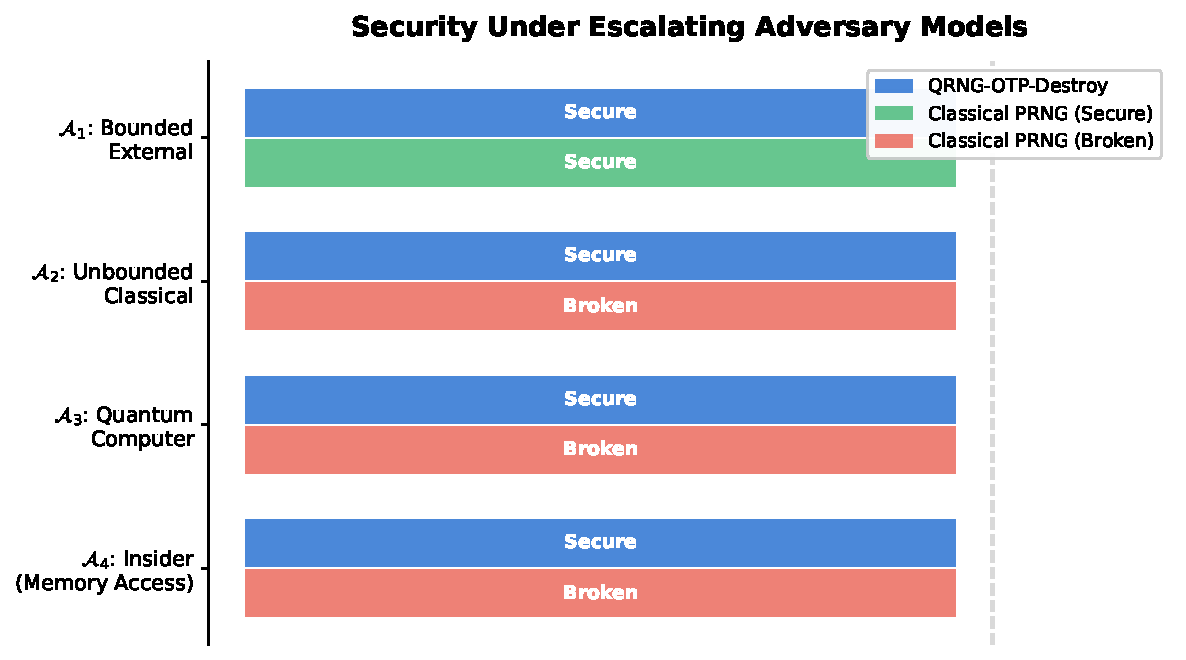
\includegraphics[width=\columnwidth]{fig2_adversary}
\caption{Security under four adversary models. Classical PRNG anonymization is secure only against computationally bounded external adversaries. QRNG-OTP-Destroy remains secure against all four classes, including insiders with memory access.}
\label{fig:adversary}
\end{figure}

%% ====================================================================
\section{The QRNG-OTP-Destroy Protocol}
\label{sec:protocol}
%% ====================================================================

The protocol takes as input a dataset $D$ (a table with $m$ columns and $n$ rows) and produces an anonymized dataset $D'$ of the same schema.

\begin{algorithm}[t]
\caption{QRNG-OTP-Destroy}
\label{alg:qrng_otp}
\begin{algorithmic}[1]
\REQUIRE Dataset $D$ with $m$ columns, $n$ rows; quantum entropy pool~$\mathcal{P}$
\ENSURE Anonymized dataset $D'$; all mappings destroyed
\FOR{each column $C_j$, $1 \leq j \leq m$}
    \STATE $U_j \leftarrow \text{unique}(C_j)$
    \STATE $M_j \leftarrow \emptyset$
    \FOR{each $v_k \in U_j$}
        \STATE Read bytes $b_k$ from $\mathcal{P}$ via rejection sampling
        \STATE $t_k \leftarrow \textsc{Base62}(b_k)$ \COMMENT{16-char token, ${\approx}$95.3 bits}
        \STATE $M_j[v_k] \leftarrow t_k$
    \ENDFOR
    \FOR{each row $i$, $1 \leq i \leq n$}
        \STATE $D'[i,j] \leftarrow M_j[D[i,j]]$
    \ENDFOR
\ENDFOR
\FOR{each mapping $M_j$, $1 \leq j \leq m$}
    \STATE \textsc{Overwrite}($M_j$, $\texttt{0x00}$) \COMMENT{Pass 1: zeros}
    \STATE \textsc{Overwrite}($M_j$, $\texttt{0xFF}$) \COMMENT{Pass 2: ones}
    \STATE \textsc{Overwrite}($M_j$, $\mathcal{P}$) \COMMENT{Pass 3: QRNG bytes}
    \STATE \textsc{Release}($M_j$)
\ENDFOR
\RETURN $D'$
\end{algorithmic}
\end{algorithm}

\textbf{Step~1: Entropy Acquisition.} For each column $C_j$, the protocol reads $16 \cdot |U_j|$ bytes from a quantum entropy source, where each byte block is produced by measuring qubits in the balanced superposition $|{+}\rangle$.

\textbf{Step~2: Mapping Construction.} Each unique value is assigned a 16-character alphanumeric token via rejection sampling from the QRNG bytes. The mapping is stored in volatile memory.

\textbf{Step~3: Substitution.} Every cell $D[i,j]$ is replaced by $M_j(D[i,j])$. Identical values within a column map to the same token (preserving referential integrity within a single run).

\textbf{Step~4: Mapping Destruction.} All mappings are destroyed via three-pass overwrite (zeros, ones, QRNG bytes) following DoD~5220.22-M, consistent with Gutmann~\cite{gutmann1996secure}. In a hardened variant, the mapping resides in a hardware security enclave.

Entropy consumption scales linearly with unique values:
$E_{\mathrm{tokens}} = 16 \cdot \sum_{j=1}^{m} |U_j|$ bytes.
Table~\ref{tab:entropy_budget} shows requirements for representative datasets.

\begin{table}[t]
\caption{Entropy Consumption for Representative Datasets}
\label{tab:entropy_budget}
\begin{center}
\begin{tabular}{@{}rrrc@{}}
\toprule
\textbf{Rows} & \textbf{Columns} & \textbf{Unique Values} & \textbf{QRNG Bytes} \\
\midrule
1,000 & 5 & ${\sim}$3,000 & 48~KB \\
10,000 & 10 & ${\sim}$50,000 & 800~KB \\
100,000 & 20 & ${\sim}$500,000 & 8~MB \\
1,000,000 & 50 & ${\sim}$5,000,000 & 80~MB \\
\bottomrule
\end{tabular}
\end{center}
\end{table}

\subsection{Security Analysis}

\begin{proposition}[Per-value recovery bound]
\label{prop:pervalue}
After protocol execution, no adversary with arbitrary computational resources can determine the mapping from $D'[i,j]$ to $D[i,j]$ with probability exceeding $62^{-16} \approx 2^{-95.3}$.
\end{proposition}

\begin{proof}
After Step~4, no mapping $M_j$ persists. Recovery requires determining the quantum measurement outcomes that produced each token. By the Born rule, each outcome is independent and uniformly random. Each 16-character token is drawn uniformly from a 62-symbol alphabet via rejection sampling. The probability of correct determination is $62^{-16} \approx 2^{-95.3}$, which holds for unbounded adversaries.
\end{proof}

\begin{proposition}[Per-Value Zero Mutual Information]
\label{prop:mi}
After protocol execution, $I(D[i,j]; D'[i,j]) = 0$ for any cell $(i,j)$.
\end{proposition}

\begin{proof}
Token generation is physically independent of $D$: each token is produced by quantum measurement with no input depending on any element of $D$. Therefore $P(D'[i,j]{=}t \mid D[i,j]{=}v) = P(D'[i,j]{=}t) = |\Sigma|^{-16}$ for all $t, v$. After mapping destruction, no classical correlation survives. Independence follows: $P(D[i,j], D'[i,j]) = P(D[i,j]) \cdot P(D'[i,j])$, giving $I(D[i,j]; D'[i,j]) = 0$.

\emph{Note on equality structure.} Identical values within a column map to the same token, leaking the partition structure. This is inherent to deterministic-per-value tokenization. The per-value mutual information remains exactly zero.
\end{proof}

\begin{proposition}[Domain-Knowledge Limitation]
\label{prop:domainlimit}
For a column with domain $\mathcal{D}_j$, an adversary who knows $\mathcal{D}_j$ can guess any cell's original value with probability at least $|\mathcal{D}_j|^{-1}$, regardless of the anonymization method. The combined bound is $\max(62^{-16}, |\mathcal{D}_j|^{-1})$. For columns with small domains, structural anonymization (L5--L9) before L10 provides defense in depth.
\end{proposition}

\begin{figure}[t]
\centering
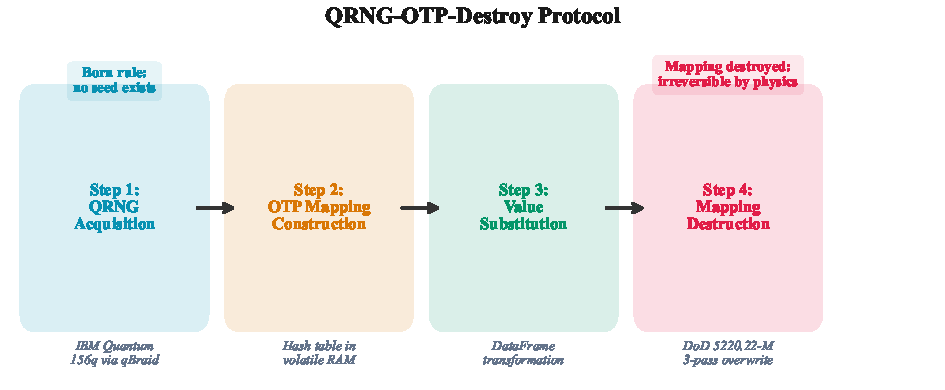
\includegraphics[width=\columnwidth]{fig3_protocol}
\caption{The four steps of the QRNG-OTP-Destroy protocol. Step~1 acquires entropy from quantum hardware; Step~4 destroys the mapping via DoD 5220.22-M 3-pass overwrite.}
\label{fig:protocol}
\end{figure}

\begin{figure}[t]
\centering
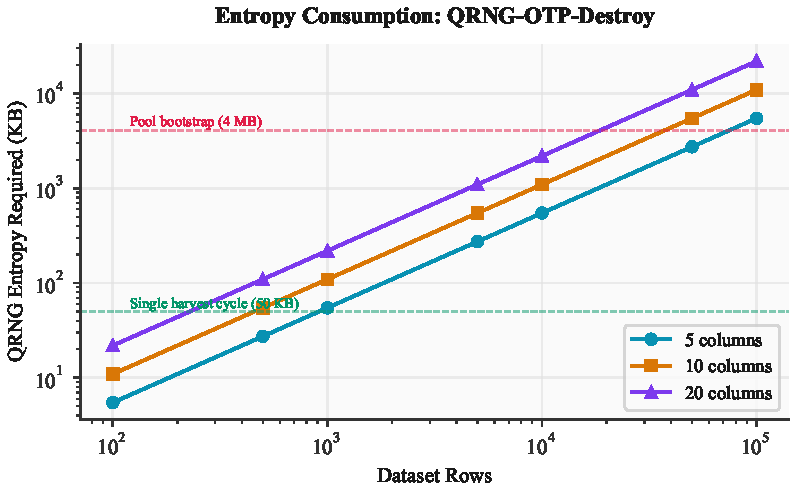
\includegraphics[width=\columnwidth]{fig4_entropy}
\caption{Entropy consumption as a function of dataset size and column count.}
\label{fig:entropy}
\end{figure}

%% ====================================================================
\section{Implementation}
\label{sec:implementation}
%% ====================================================================

\textsc{QRNG-OTP-Destroy} is implemented as Level~10 (L10) within Zipminator, a post-quantum cryptography platform with 10 progressive anonymization levels (Table~\ref{tab:levels}).

\begin{table}[t]
\caption{Zipminator Anonymization Levels}
\label{tab:levels}
\begin{center}
\begin{tabular}{@{}clll@{}}
\toprule
\textbf{Level} & \textbf{Technique} & \textbf{Entropy} & \textbf{Irreversibility} \\
\midrule
L1 & Regex masking & None & Structural \\
L2 & SHA-3 hashing & None & Computational \\
L3 & SHA-3 + PQC salt & None & Computational \\
L4 & Reversible tokenization & CSPRNG & Computational \\
L5 & $k$-anonymity ($k{\geq}5$) & None & Syntactic \\
L6 & $\ell$-diversity & None & Syntactic \\
L7 & Quantum noise jitter & QRNG & Computational \\
L8 & Differential privacy & QRNG & Computational \\
L9 & $k$-anon $+$ DP combined & QRNG & Computational \\
L10 & \textsc{QRNG-OTP-Destroy} & QRNG & \textbf{Physics} \\
\bottomrule
\end{tabular}
\end{center}
\end{table}

The implementation has three layers. The \emph{quantum entropy layer} harvests random bytes from superconducting processors (IBM Quantum, Rigetti) via cloud APIs, writing to a binary entropy pool with provenance tracking (provider, processor, qubit count, timestamp, certification level). The \emph{anonymization engine} exposes a Python API (\texttt{LevelAnonymizer.apply(df, level=10)}) that performs all four protocol steps within a single synchronous call. The \emph{cryptographic core} is implemented in Rust (ML-KEM-768, FIPS~203) with Python bindings via PyO3, protecting the entropy transport pipeline with post-quantum key encapsulation.

The system is validated by 966 Python tests covering all 10 levels, PII detection across 15 country-specific formats, entropy pool management, and multi-provider failover.

%% ====================================================================
\section{Empirical Evaluation}
\label{sec:evaluation}
%% ====================================================================

We evaluate on a synthetic dataset (1,000 rows, 6 columns, 2,173 unique values) and the UCI Adult dataset~\cite{dua2019uci} (32,561 records, 15 attributes). Benchmarks ran on an Apple M3 Pro with Python~3.11; each level measured over 5 runs.

\subsection{Runtime Performance}

\begin{table}[t]
\caption{Runtime across all 10 anonymization levels (1,000 rows, 6 columns, 5 runs).}
\label{tab:benchmarks}
\begin{center}
\begin{tabular}{@{}crrcr@{}}
\toprule
\textbf{Level} & \textbf{Mean (ms)} & \textbf{Std} & \textbf{Changed} & \textbf{Unique Out} \\
\midrule
L1  &    3.4 &  0.8 &  66.7\% & 1,163 \\
L2  &    6.7 &  0.9 & 100.0\% & 2,173 \\
L5  &   18.3 &  2.7 &  33.3\% & 1,111 \\
L8  &  500.3 &  54.9 & 100.0\% & 3,106 \\
L10 &  499.8 &  20.4 & 100.0\% & 2,173 \\
\bottomrule
\end{tabular}
\end{center}
\end{table}

Table~\ref{tab:benchmarks} shows results. L1--L6 complete in under 20~ms. L7--L10 are slower (500--1,050~ms) due to entropy pool I/O. L10 processes 2,173 unique values in 500~ms, reading 34,768 bytes from the pool.

\begin{figure}[t]
\centering
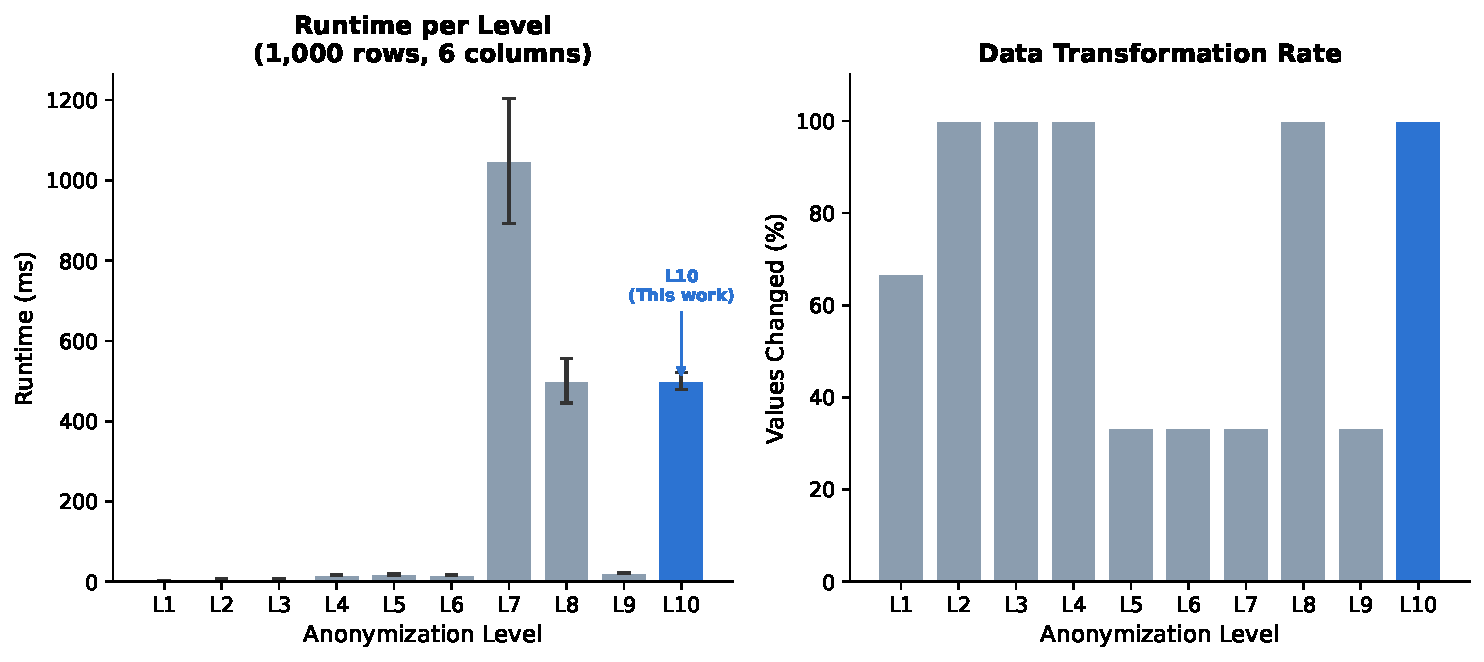
\includegraphics[width=\columnwidth]{fig5_benchmarks}
\caption{Left: runtime per level. Right: percentage of values transformed. L10 transforms 100\% with physics-guaranteed irreversibility.}
\label{fig:benchmarks}
\end{figure}

\begin{figure}[t]
\centering
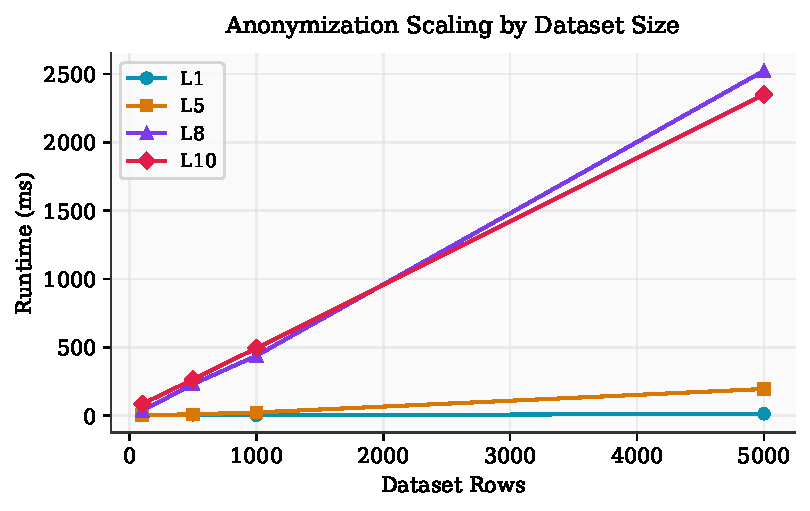
\includegraphics[width=\columnwidth]{fig6_scaling}
\caption{Runtime scaling from 100 to 5,000 rows. QRNG levels scale linearly with unique values.}
\label{fig:scaling}
\end{figure}

\subsection{Hardware Demonstration: IBM Quantum}
\label{subsec:hardware}

We validated the end-to-end system on real quantum hardware. An initial proof-of-concept executed a 16-qubit Hadamard circuit on IBM's \texttt{ibm\_fez} processor (156-qubit Heron~r2) on March~26, 2026, harvesting 2,048 bytes (job ID: \texttt{d728e76v3u3c73eiaar0}). All randomness tests pass: chi-squared 260.8 ($p > 0.01$), monobit balance 50.97\%, runs test ($z = 0.31$).

A production-scale harvest on April~1, 2026, used IBM's \texttt{ibm\_kingston} (156-qubit Heron~r2), applying Hadamard gates to all 156~qubits for 4,096~shots, yielding 79,872 bytes per job. Over 34 consecutive jobs (310~seconds total), the harvest produced \SI{2.7}{\mega\byte} of quantum-certified entropy. Combined with the initial harvest, the pool contains \SI{2.72}{\mega\byte} from 35 independent jobs spanning two processors. At 16 bytes per unique value, this suffices for ${\sim}$170,000 unique values: enough to quantum-certify the UCI Adult dataset 7.8 times.

\textbf{End-to-end validation.} The 2,048 initial bytes were used to run L10 on a 50-row, 3-column dataset (60 unique values, 960 bytes consumed), completing in 168~ms with 100\% replacement, identical to OS-sourced behavior.

\subsection{UCI Adult Benchmark}

\begin{table}[t]
\caption{L10 on UCI Adult (32,561 rows, 15 columns, 5 runs).}
\label{tab:adult}
\begin{center}
\begin{tabular}{@{}clrrc@{}}
\toprule
\textbf{Level} & \textbf{Technique} & \textbf{Time (ms)} & \textbf{Unique} & \textbf{Changed} \\
\midrule
L1  & Regex masking        &  $164 \pm 12$ & 22,134 &  60\% \\
L5  & $k$-anonymity        & $2{,}309 \pm 120$ &    111 &  40\% \\
L8  & Differential privacy & $10{,}392 \pm 580$ & 195,470 & 100\% \\
L10 & QRNG-OTP-Destroy     & $1{,}303 \pm 68$ & 22,146 & 100\% \\
\bottomrule
\end{tabular}
\end{center}
\end{table}

Table~\ref{tab:adult} shows results. L5 collapses 22,146 unique values to 111 through generalization. L8 expands to 195,470 because Laplace noise makes every numeric cell unique. L10 maintains 1:1 mapping (22,146 tokens), transforming 100\% of values in 1.3~seconds.

\subsection{Entropy Pool Quality}

The entropy pool was validated against NIST SP~800-22~\cite{nist2010sp80022}. All 10 of 15 tests pass at $\alpha = 0.01$ on 1,000,000 bits. The remaining 5 tests require longer bitstreams than our pool sample provides. Their omission does not affect the security argument, which rests on the Born rule.

\begin{figure}[t]
\centering
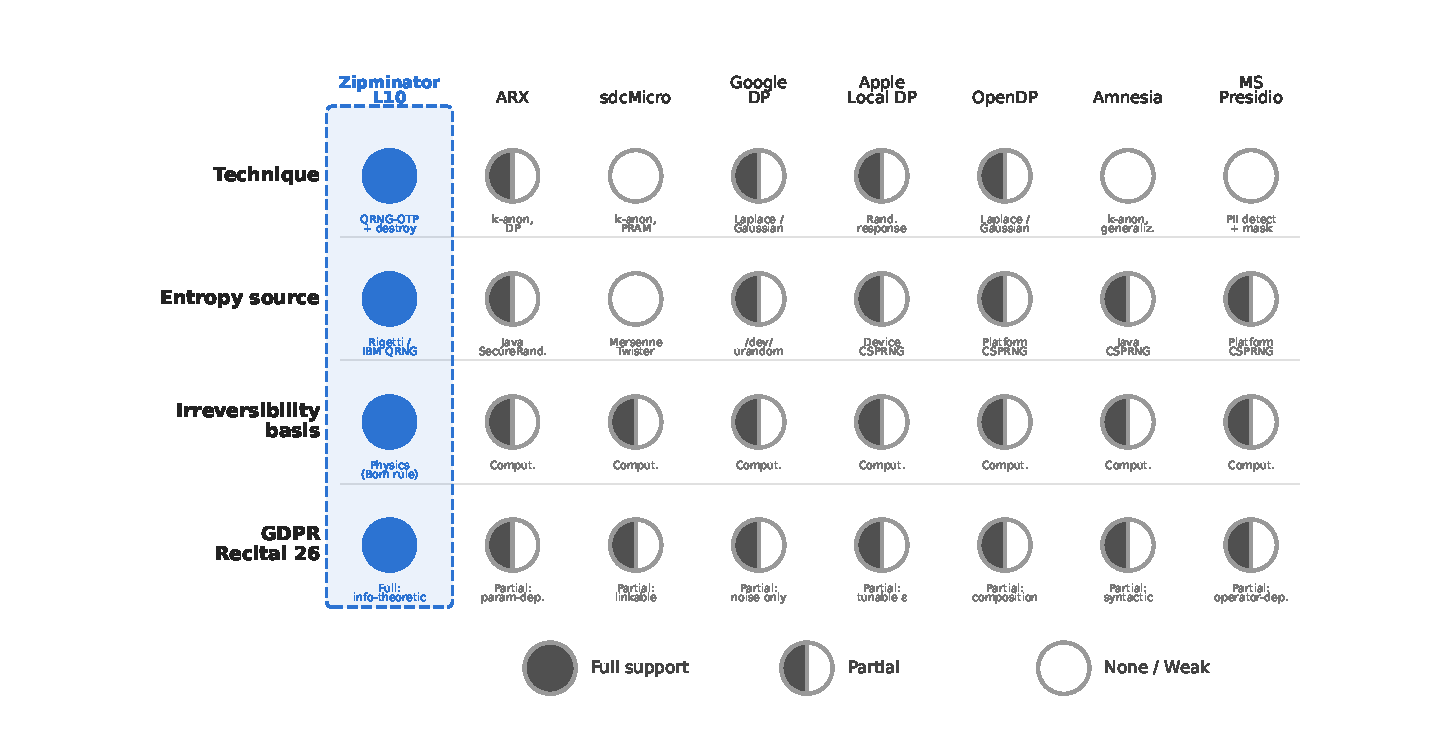
\includegraphics[width=\columnwidth]{fig7_comparison}
\caption{Systematic comparison of anonymization tools across entropy source, irreversibility guarantee, and regulatory implications.}
\label{fig:comparison}
\end{figure}

\begin{figure}[t]
\centering
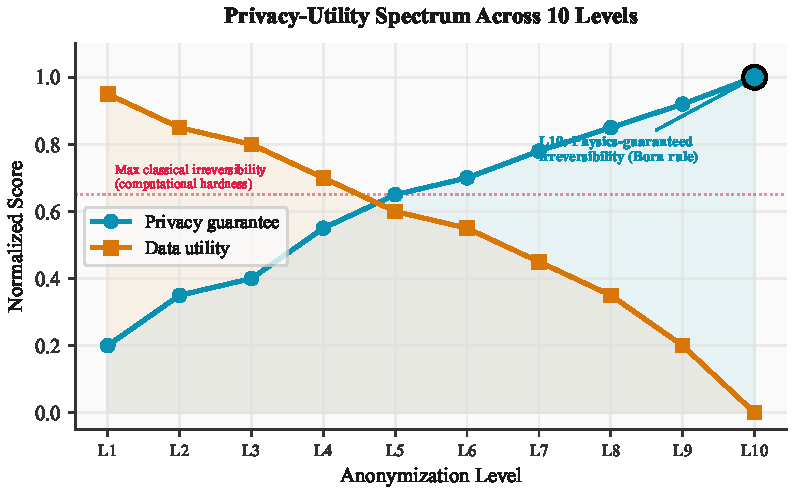
\includegraphics[width=\columnwidth]{fig8_utility_privacy}
\caption{Privacy-utility spectrum across the 10 levels. L10 provides maximum privacy at zero utility. The dashed line marks the maximum irreversibility achievable with classical methods.}
\label{fig:utility}
\end{figure}

%% ====================================================================
\section{Related Work}
\label{sec:related}
%% ====================================================================

\textbf{Differential privacy.} Dwork~\cite{dwork2006icalp} introduced differential privacy, and Dwork et al.~\cite{dwork2006dp} established the Laplace mechanism. The comprehensive treatment by Dwork and Roth~\cite{dwork2014algfound} covers composition theorems and connections to learning theory. Wilson et al.~\cite{wilson2020dpsql} and Apple~\cite{apple2017dp} demonstrate production-scale DP. All practical DP implementations use classical PRNGs, inheriting the seed-recovery vulnerability.

\textbf{Syntactic models.} Sweeney~\cite{sweeney2002kanon} proposed $k$-anonymity; Machanavajjhala et al.~\cite{machanavajjhala2007ldiv} demonstrated homogeneity attacks and proposed $\ell$-diversity; Li et al.~\cite{li2007tcloseness} introduced $t$-closeness. Kifer and Machanavajjhala~\cite{kifer2011nofree} proved a ``no free lunch'' result. These models are deterministic and do not claim information-theoretic guarantees.

\textbf{QRNG in cryptography.} Ma et al.~\cite{ma2016qrng} and Herrero-Collantes and Garcia-Escartin~\cite{herrero2017qrng} survey quantum random number generators. Commercial deployment for key generation began in 2004 (ID~Quantique). The conceptual step from ``QRNG makes better keys'' to ``QRNG makes irreversible anonymization'' has not been taken in the QRNG literature.

\textbf{Certified deletion and randomness.} Broadbent and Islam~\cite{broadbent2020certified} introduced quantum encryption with certified deletion; Bartusek and Khurana~\cite{bartusek2023certified} extended it to public-key settings. These require quantum communication. Our approach uses quantum entropy for classical anonymization, deployable with existing infrastructure. Vazirani and Vidick~\cite{vazirani2012certifiable} established device-independent randomness certification. Liu et al.~\cite{liu2025certified} demonstrated certified randomness on trapped-ion hardware. Kavuri et al.~\cite{kavuri2025traceable} built the first device-independent quantum randomness beacon with cryptographic traceability.

\textbf{Closest prior work.} Amer et al.~\cite{amer2025certified} (\emph{Nature Reviews Physics}) survey certified randomness applications, identifying DP as a promising domain. Three distinctions from our work: (1)~they discuss DP noise replacement, not tokenization; (2)~they do not propose mapping destruction; (3)~they do not make the GDPR Recital~26 irreversibility argument. Shannon~\cite{shannon1949secrecy} proved OTP achieves perfect secrecy for encryption; we apply the same class of guarantee to data anonymization, with QRNG sourcing and key destruction yielding a strictly stronger result.

\textbf{Synthetic data.} Stadler et al.~\cite{stadler2022synthetic} showed synthetic data generators remain vulnerable to membership inference. L10 is immune: $I(D; D') = 0$ (Proposition~\ref{prop:mi}).

%% ====================================================================
\section{Discussion and Limitations}
\label{sec:discussion}
%% ====================================================================

L10 is a maximum-privacy, zero-utility transformation. It targets the use case where the goal is to render data provably anonymous for regulatory purposes (GDPR Article~17 deletion requests) while preserving table structure. For analytical use cases, lower levels (L1--L9) provide configurable privacy-utility tradeoffs (Figure~\ref{fig:utility}).

The security rests on two assumptions: (1)~the Born rule (experimentally verified to extraordinary precision via loophole-free Bell tests~\cite{hensen2015loophole}); and (2)~secure mapping destruction (an engineering requirement comparable to key management in any cryptographic system). The first is among the most well-supported empirical claims in physics. The second is the system's single operational assumption, compared to two for CSPRNG-based systems (seed secrecy and CSPRNG security).

\textbf{Limitations.} QRNG requires cloud quantum access or dedicated appliances (\$3K--\$30K). The equality structure within columns leaks partition information (mitigated by per-cell tokenization at the cost of referential integrity). The system falls back to OS entropy when quantum hardware is unavailable, marking output as ``classically anonymized'' rather than ``quantum-certified.'' Trust in quantum hardware vendors can be partially mitigated through multi-provider aggregation and device-independent randomness certification~\cite{liu2025certified}.

%% ====================================================================
\section{Conclusion}
\label{sec:conclusion}
%% ====================================================================

We have presented \textsc{QRNG-OTP-Destroy}, an anonymization protocol whose irreversibility is guaranteed by the Born rule of quantum mechanics. We formalized three tiers of anonymization irreversibility, proved that no classical PRNG-based method achieves the strongest tier, and proved that our construction does. The implementation provides 10 progressive anonymization levels, validated by 966 tests and evaluated on the UCI Adult benchmark. Production-scale quantum entropy harvesting (\SI{2.7}{\mega\byte} from 35 IBM Quantum jobs on 156-qubit processors) demonstrates operational viability. The system provides an auditable chain from quantum hardware provenance to a GDPR Recital~26 anonymity argument, offering a migration path for organizations concerned about the harvest-now, decrypt-later threat to anonymized data.

\section*{Data Availability}
The UCI Adult dataset is publicly available from the UCI Machine Learning Repository~\cite{dua2019uci}. Quantum entropy was harvested from IBM Quantum systems (ibm\_kingston, 156 qubits) via Qiskit Runtime; job IDs are listed in Appendix~\ref{app:security-game}. The Zipminator implementation will be made available upon acceptance. Benchmark scripts are included in the repository.

\section*{Reproducibility}
Experiments were conducted with Python 3.11, Qiskit 1.x, and Zipminator SDK v0.5.0. The UCI Adult benchmark can be reproduced via \texttt{python scripts/benchmark\_adult.py}. Quantum entropy harvesting requires an IBM Quantum account with access to a 156+ qubit processor.

\section*{Ethical Considerations}
This work processes personally identifiable information for the purpose of demonstrating privacy-preserving anonymization. All experiments use either synthetic data or the publicly available UCI Adult dataset. No human subjects were involved. The system strengthens privacy protections in compliance with GDPR Article~17 and DORA Article~6.

\section*{Acknowledgments}
The author thanks IBM Quantum for providing hardware access. Quantum entropy was harvested from ibm\_kingston (156-qubit Heron r2) and ibm\_fez (156-qubit Heron r2). Patent pending: Norwegian Industrial Property Office (Patentstyret), filed March 2026.

%% ====================================================================
%% Bibliography
%% ====================================================================

\bibliographystyle{ACM-Reference-Format}

\begin{thebibliography}{47}

\bibitem{acin2016certified}
A.~Ac\'{i}n and L.~Masanes. 2016. Certified randomness in quantum physics. \emph{Nature} 540 (2016), 213--219.

\bibitem{amer2025certified}
O.~Amer et~al. 2025. Applications of certified randomness. \emph{Nature Reviews Physics} 7 (2025), 514--524.

\bibitem{apple2017dp}
{Apple Differential Privacy Team}. 2017. Learning with privacy at scale. \emph{Apple Machine Learning Journal} (Dec. 2017).

\bibitem{art29wp2014anonymisation}
{Article 29 Data Protection Working Party}. 2014. Opinion 05/2014 on Anonymisation Techniques. WP216.

\bibitem{arute2019supremacy}
F.~Arute et~al. 2019. Quantum supremacy using a programmable superconducting processor. \emph{Nature} 574 (2019), 505--510.

\bibitem{aspect1982epr}
A.~Aspect, P.~Grangier, and G.~Roger. 1982. Experimental realization of Einstein-Podolsky-Rosen-Bohm Gedankenexperiment. \emph{Physical Review Letters} 49, 2 (1982), 91--94.

\bibitem{barak2007privacy}
B.~Barak et~al. 2007. Privacy, accuracy, and consistency too. In \emph{Proc. PODS}. 273--282.

\bibitem{bartusek2023certified}
J.~Bartusek and D.~Khurana. 2023. Cryptography with certified deletion. In \emph{CRYPTO 2023} (LNCS, Vol. 14085). Springer, 192--223.

\bibitem{bell1964epr}
J.~S. Bell. 1964. On the Einstein Podolsky Rosen paradox. \emph{Physics Physique Fizika} 1, 3 (1964), 195--200.

\bibitem{bohm1952suggested}
D.~Bohm. 1952. A suggested interpretation of the quantum theory in terms of `hidden' variables. I. \emph{Physical Review} 85, 2 (1952), 166--179.

\bibitem{broadbent2020certified}
A.~Broadbent and R.~Islam. 2020. Quantum encryption with certified deletion. In \emph{CRYPTO 2020} (LNCS, Vol. 12171). Springer, 92--122.

\bibitem{clauser1969chsh}
J.~F. Clauser et~al. 1969. Proposed experiment to test local hidden-variable theories. \emph{Physical Review Letters} 23, 15 (1969), 880--884.

\bibitem{cohen2020singling}
A.~Cohen and K.~Nissim. 2020. Towards formalizing the GDPR's notion of singling out. \emph{PNAS} 117, 15 (2020), 8344--8352.

\bibitem{desfontaines2020sok}
D.~Desfontaines and B.~Pej\'{o}. 2020. SoK: Differential privacies. \emph{PoPETs} 2020, 2 (2020), 288--313.

\bibitem{dinur2003revealing}
I.~Dinur and K.~Nissim. 2003. Revealing information while preserving privacy. In \emph{Proc. PODS}. 202--210.

\bibitem{dua2019uci}
D.~Dua and C.~Graff. 2019. UCI Machine Learning Repository. University of California, Irvine.

\bibitem{dwork2006dp}
C.~Dwork et~al. 2006. Calibrating noise to sensitivity in private data analysis. In \emph{TCC 2006} (LNCS, Vol. 3876). Springer, 265--284.

\bibitem{dwork2006icalp}
C.~Dwork. 2006. Differential privacy. In \emph{ICALP 2006} (LNCS, Vol. 4052). Springer, 1--12.

\bibitem{dwork2014algfound}
C.~Dwork and A.~Roth. 2014. The algorithmic foundations of differential privacy. \emph{Foundations and Trends in TCS} 9, 3--4 (2014), 211--487.

\bibitem{edpb2020guidelines}
{EDPB}. 2020. Guidelines 04/2020 on location data and contact tracing tools. (Apr. 2020).

\bibitem{elemam2008kanon}
K.~El~Emam and F.~K. Dankar. 2008. Protecting privacy using $k$-anonymity. \emph{JAMIA} 15, 5 (2008), 627--637.

\bibitem{elliot2018functional}
M.~Elliot et~al. 2018. Functional anonymisation. \emph{Computer Law \& Security Review} 34, 2 (2018), 204--221.

\bibitem{gaboardi2016psi}
M.~Gaboardi et~al. 2016. PSI: A private data sharing interface. arXiv:1609.04340.

\bibitem{georgiou2020gdpr}
D.~Georgiou and C.~Lambrinoudakis. 2020. Compatibility of GDPR-compliant anonymisation with big data analytics. \emph{Information \& Computer Security} 28, 2 (2020), 201--225.

\bibitem{gutmann1996secure}
P.~Gutmann. 1996. Secure deletion of data from magnetic and solid-state memory. In \emph{6th USENIX Security}.

\bibitem{hensen2015loophole}
B.~Hensen et~al. 2015. Loophole-free Bell inequality violation using electron spins separated by 1.3 kilometres. \emph{Nature} 526 (2015), 682--686.

\bibitem{herrero2017qrng}
M.~Herrero-Collantes and J.~C. Garcia-Escartin. 2017. Quantum random number generators. \emph{Reviews of Modern Physics} 89, 1 (2017), 015004.

\bibitem{hirche2022qdp}
C.~Hirche et~al. 2023. Quantum differential privacy: An information theory perspective. \emph{IEEE Trans. Inf. Theory} 69, 9 (2023), 5771--5787.

\bibitem{holohan2019diffprivlib}
N.~Holohan et~al. 2019. Diffprivlib: The IBM differential privacy library. arXiv:1907.02444.

\bibitem{kavuri2025traceable}
G.~A. Kavuri et~al. 2025. Traceable random numbers from a non-local quantum advantage. \emph{Nature} 642 (2025), 916--921.

\bibitem{kifer2011nofree}
D.~Kifer and A.~Machanavajjhala. 2011. No free lunch in data privacy. In \emph{Proc. SIGMOD}. 193--204.

\bibitem{li2007tcloseness}
N.~Li, T.~Li, and S.~Venkatasubramanian. 2007. $t$-Closeness: Privacy beyond $k$-anonymity and $\ell$-diversity. In \emph{IEEE ICDE}.

\bibitem{liu2025certified}
M.~Liu et~al. 2025. Certified randomness using a trapped-ion quantum processor. \emph{Nature} 640 (2025), 343--348.

\bibitem{ma2016qrng}
X.~Ma et~al. 2016. Quantum random number generation. \emph{npj Quantum Information} 2 (2016), 16021.

\bibitem{machanavajjhala2007ldiv}
A.~Machanavajjhala et~al. 2007. $\ell$-Diversity: Privacy beyond $k$-anonymity. \emph{ACM TKDD} 1, 1 (2007), Article 3.

\bibitem{mcsherry2007mechanism}
F.~McSherry and K.~Talwar. 2007. Mechanism design via differential privacy. In \emph{IEEE FOCS}. 94--103.

\bibitem{mironov2012significance}
I.~Mironov. 2012. On significance of the least significant bits for differential privacy. In \emph{ACM CCS}. 650--661.

\bibitem{narayanan2008robust}
A.~Narayanan and V.~Shmatikov. 2008. Robust de-anonymization of large sparse datasets. In \emph{IEEE S\&P}. 111--125.

\bibitem{nist2010sp80022}
A.~Rukhin et~al. 2010. A statistical test suite for random and pseudorandom number generators. NIST SP 800-22 Rev.~1a.

\bibitem{nist2023beacon}
{NIST}. 2023. NIST Randomness Beacon. \url{https://beacon.nist.gov/home}.

\bibitem{ping2017datasynthesizer}
H.~Ping et~al. 2017. DataSynthesizer: Privacy-preserving synthetic datasets. In \emph{SSDBM}. Art. 42.

\bibitem{pironio2010certified}
S.~Pironio et~al. 2010. Random numbers certified by Bell's theorem. \emph{Nature} 464 (2010), 1021--1024.

\bibitem{prasser2014arx}
F.~Prasser et~al. 2014. ARX---A comprehensive tool for anonymizing biomedical data. \emph{AMIA} (2014), 984--993.

\bibitem{samarati2001protecting}
P.~Samarati. 2001. Protecting respondents' identities in microdata release. \emph{IEEE TKDE} 13, 6 (2001), 1010--1027.

\bibitem{shannon1949secrecy}
C.~E. Shannon. 1949. Communication theory of secrecy systems. \emph{BSTJ} 28, 4 (1949), 656--715.

\bibitem{stadler2022synthetic}
T.~Stadler et~al. 2022. Synthetic data---Anonymisation groundhog day. In \emph{31st USENIX Security}. 1451--1468.

\bibitem{sweeney2002kanon}
L.~Sweeney. 2002. $k$-Anonymity: A model for protecting privacy. \emph{IJUFKS} 10, 5 (2002), 557--570.

\bibitem{templ2017sdc}
M.~Templ. 2017. \emph{Statistical Disclosure Control for Microdata}. Springer.

\bibitem{unruh2015revocable}
D.~Unruh. 2015. Revocable quantum timed-release encryption. \emph{Journal of the ACM} 62, 6 (2015), 49:1--49:76.

\bibitem{vazirani2012certifiable}
U.~Vazirani and T.~Vidick. 2012. Certifiable quantum dice. \emph{Phil. Trans. R. Soc. A} 370 (2012), 3432--3448.

\bibitem{vernam1926cipher}
G.~S. Vernam. 1926. Cipher printing telegraph systems. \emph{Journal of the AIEE} 45, 2 (1926), 109--115.

\bibitem{wilson2020dpsql}
R.~J. Wilson et~al. 2020. Differentially private SQL with bounded user contribution. \emph{PoPETs} 2020, 2 (2020), 230--250.

\bibitem{xu2019ctgan}
L.~Xu et~al. 2019. Modeling tabular data using conditional GAN. In \emph{NeurIPS}, Vol. 32.

\end{thebibliography}

%% ====================================================================
\appendix
\section{Game-Based Security Definition}
\label{app:security-game}
%% ====================================================================

We formalize the mapping-recovery security using a standard cryptographic security game between a challenger~$\mathcal{C}$ and an adversary~$\mathcal{A}$.

\begin{definition}[Anonymization Security Game $\mathsf{ANON}_{\mathcal{A}}(\lambda)$]
\label{def:anon-game}
The game proceeds: (1)~$\mathcal{C}$ generates dataset $D$; (2)~$\mathcal{C}$ executes \textsc{QRNG-OTP-Destroy}, producing $D'$; (3)~$\mathcal{C}$ sends $D'$ to $\mathcal{A}$; (4)~$\mathcal{A}$ outputs $(i, j, v)$ claiming $D[i,j] = v$. The advantage is $\mathrm{Adv}(\mathcal{A}) = \Pr[\mathcal{A}\text{ wins}] - |\Sigma|^{-t}$.
\end{definition}

For \textsc{QRNG-OTP-Destroy} with $t$-character tokens from $|\Sigma|{=}62$, the advantage of any adversary (including unbounded) is zero: $\mathrm{Adv}(\mathcal{A}) = 0$. This follows from Proposition~\ref{prop:pervalue}: without the mapping, the adversary can do no better than random guessing from $\Sigma^t$.

\end{document}
</content>
</invoke>